
\subsection{Audioserialisierer}\label{subsec:Audio_Serializer}

Für die Übertragung der Audiodaten zum Codec ist der \textit{Audioserialisierer} zuständig. Obwohl es von Intel bereits eine IP gäbe, um diese Übertragung zu übernehmen, mussten wir diese Komponente nochmals selber schreiben. Der zur Verfügung gestellte IP Core benötigt eine spezifische Clockfrequenz von \SI{12.288}{MHz}. Jedoch müssen die Tonhöhenverarbeitung und der Serialisierer Clocks erhalten, die denselben Referenzclock besitzen, um nicht Daten zu verlieren. Die verlangten Clockfrequenzen von \SI{54}{MHz} für die Tonhöhenverarbeitung und die zuvor genannten \SI{12.288}{MHz} können nicht in einem PLL generiert werden. \\
Wie der Name der Komponente schon sagt, serialisiert sie die parallelen Daten für die Übertragung. Dabei sieht der geforderte Signalverlauf des Codec wie in Abbildung \ref{img:Codec_Signals} dargestellt aus. Der Audioserialisierer gibt jeweils für den linken und rechten Kanal dieselben Daten aus. Die Signale DACLRC und BCLK werden vom Codec nach der Konfiguration, beschrieben in Kapitel \ref{subsec:audio}, vom Codec generiert und sind Eingänge des Audioserialisierers. Bei jeder positiven Flanke von DACLRC lädt der Serialisierer einen neuen Audiosignalwert ins Schieberegister und schiebt bei jeder negativen Flanke des BCLK ein neues Bit ins Signal DACDAT.

Die Komponente Audioserialisierer ist in der Datei \textit{audio\_serializer.vhd} zu finden.

\begin{figure}[t]
	\centering
	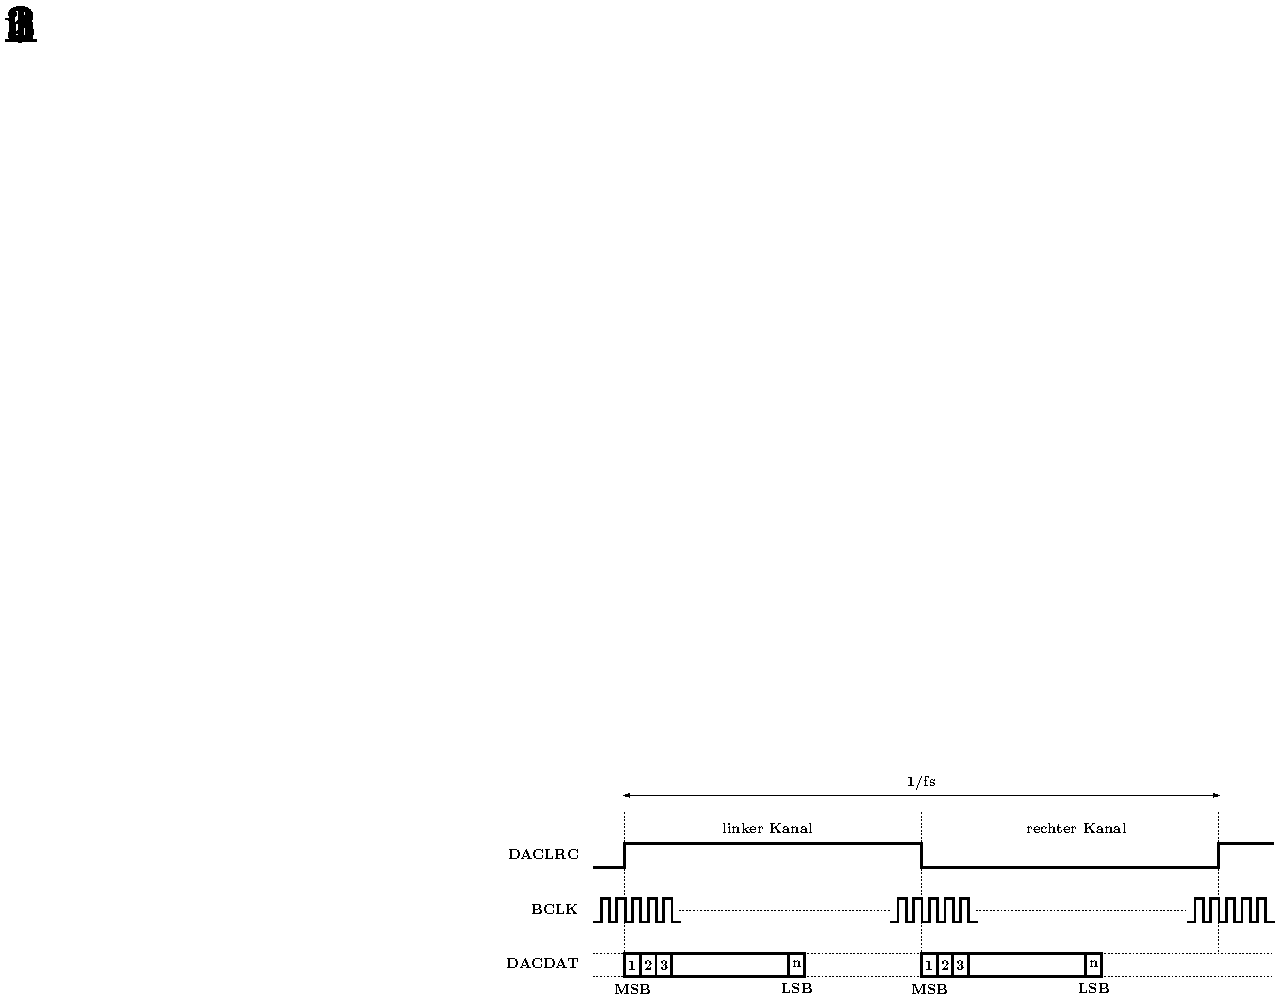
\includegraphics[width=\textwidth]{Codec_Signals_Serializer.pdf}
	\caption{Signalverlauf des Codec Interface} 
	\label{img:Codec_Signals}
\end{figure}  